% Paquets généraux
\documentclass[a4paper,12pt,titlepage,twoside]{article}
\usepackage[T1]{fontenc}
\usepackage[utf8]{inputenc}
\usepackage[french]{babel}
\usepackage{subcaption}
\addto\captionsfrench{%
  \renewcommand{\tablename}{Tableau}%
}
\usepackage[gen]{eurosym}
%\usepackage[dvips]{graphicx}
\usepackage{minted}
\usepackage{fancyhdr}
\usepackage{pdfpages} 
\usepackage{multido}
\usepackage{hyperref}
\usepackage{textcomp}
\usepackage{schemabloc}
%\usepackage[bitstream-charter]{mathdesign}
\usepackage{array}
\newcolumntype{P}[1]{>{\centering\arraybackslash}p{#1}}
\usepackage[shortlabels]{enumitem}
\usepackage[framemethod=TikZ]{mdframed}

\newcommand{\id}{71}
\newcommand{\nom}{Théorie des mécanismes}
\newcommand{\sequence}{04}
\newcommand{\nomsequence}{Liaisons entre les solides}
\newcommand{\num}{02}
\newcommand{\type}{KH}
\newcommand{\descrip}{Liaisons équivalentes, hyperstatisme, liaisons en série et en parallèle, théorie des graphes}
\newcommand{\competences}{B2-12: Proposer une modélisation des liaisons avec leurs caractéristiques géométriques. \\ &  B2-13: Proposer un modèle cinématique paramétré à partir d'un système réel, d'une maquette numérique ou d'u \\ &  B2-17: Simplifier un modèle de mécanisme. \\ &  B2-18: Modifier un modèle pour le rendre isostatique. \\ &  C1-04: Proposer une démarche permettant d'obtenir une loi entrée-sortie géométrique.  \\ &  C2-05: Caractériser le mouvement d'un repère par rapport à un autre repère. \\ &  C2-06: Déterminer les relations entre les grandeurs géométriques ou cinématiques. }
\newcommand{\nbcomp}{7}
\newcommand{\systemes}{}
\newcommand{\systemesnum}{}
\newcommand{\systemessansaccent}{}
\newcommand{\ilot}{2}
\newcommand{\ilotstr}{02}
\newcommand{\dossierilot}{\detokenize{Ilot_02 }}

%\usepackage{style}
\usepackage{bodegraph}
\usepackage{rpcinematik}
\usepackage[locale = FR]{siunitx}
\usepackage{caption}
\newcommand{\institute}{Lycée Dorian}

\usepackage{listings}
\usepackage{fancyvrb}
\usepackage{color}
\usepackage{xcolor}
\usepackage{colortbl}
\usepackage{helvet}
\usepackage[frenchmath]{newtxsf} % for sans serif symbols
\renewcommand{\familydefault}{\sfdefault}
%\usepackage{amsfonts}
%\usepackage{amsmath}
%\usepackage{lmodern}
\usepackage{mathastext}
%\usepackage{xspace}
\usepackage{varioref}
\usepackage{tabularx}
%\usepackage{floatflt}
\usepackage{graphics}
\usepackage{wrapfig}
\usepackage{textcomp}
\usepackage{tikz,tkz-tab}
\usepackage[european resistor, european voltage, european current]{circuitikz}
\usepackage{wrapfig}
\usepackage{gensymb}
\usepackage[percent]{overpic}
\usetikzlibrary{babel}
\usepackage{ifthen}
\usepackage{cancel}
\usepackage{etoolbox}
\usepackage{multirow}
%\usepackage{boxedminipage}
\definecolor{gris25}{gray}{0.75}
\definecolor{bleu}{RGB}{18,33,98}
\definecolor{bleuf}{RGB}{42,94,171}
\definecolor{bleuc}{RGB}{231,239,247}
\definecolor{bleum}{RGB}{160,195,226}
\definecolor{rougef}{RGB}{185,18,27}
\definecolor{rougec}{RGB}{255,188,204}%255,230,231
\definecolor{vertf}{RGB}{103,126,82}
\definecolor{vertc}{RGB}{220,255,191}
\definecolor{forestgreen}{rgb}{0.13,0.54,0.13}
\definecolor{blcr}{rgb}{0.59,0.69,0.84}
\definecolor{blfr}{rgb}{0.32,0.51,0.75}
\definecolor{orfr}{rgb}{0.90,0.42,0.15}
\definecolor{orcr}{rgb}{0.90,0.65,0.50}
\definecolor{orangef}{rgb}{0.659,0.269,0.072}
\definecolor{orange}{rgb}{0.58,0.35,0.063}
\definecolor{orangec}{rgb}{0.43,0.32,0.25}
\definecolor{rcorrect}{rgb}{0.6,0,0}
\definecolor{sequence}{rgb}{0.75,0.75,0.75}
\definecolor{competences}{rgb}{0.61,0.73,0.35}
\definecolor{rose}{HTML}{ff00ff}
\definecolor{grisf}{HTML}{222222}
\definecolor{grisc}{HTML}{636363}
\definecolor{normal}{HTML}{4087c4}
\definecolor{info}{HTML}{5bc0de}
\definecolor{success}{RGB}{92,184,92}
\definecolor{warning}{RGB}{240,173,78}
\definecolor{danger}{RGB}{217,83,79}
\hypersetup{                    % parametrage des hyperliens
    colorlinks=true,                % colorise les liens
    breaklinks=true,                % permet les retours à la ligne pour les liens trop longs
    urlcolor= blfr,                 % couleur des hyperliens
    linkcolor= orange,                % couleur des liens internes aux documents (index, figures, tableaux, equations,...)
    citecolor= forestgreen                % couleur des liens vers les references bibliographiques
    }

\newcolumntype{M}[1]{>{\centering\arraybackslash}m{#1}}
\definecolor{codegreen}{rgb}{0,0.6,0}
\definecolor{codegray}{rgb}{0.5,0.5,0.5}
\definecolor{codepurple}{rgb}{0.58,0,0.82}
\definecolor{backcolour}{rgb}{0.95,0.95,0.92}

\lstdefinestyle{mystyle}{
    backgroundcolor=\color{backcolour},   
    commentstyle=\color{codegreen},
    keywordstyle=\color{magenta},
    numberstyle=\tiny\color{codegray},
    stringstyle=\color{codepurple},
    basicstyle=\ttfamily\footnotesize,
    breakatwhitespace=false,         
    breaklines=true,                 
    captionpos=b,                    
    keepspaces=true,                 
    numbers=left,                    
    numbersep=5pt,                  
    showspaces=false,                
    showstringspaces=false,
    showtabs=false,                  
    tabsize=2
}

\lstset{style=mystyle}

% Mise en page
\pagestyle{fancy}

\setlength{\hoffset}{-18pt}
\setlength{\oddsidemargin}{0pt} 	% Marge gauche sur pages impaire2s
\setlength{\evensidemargin}{0pt} 	% Marge gauche sur pages paires
\setlength{\marginparwidth}{00pt} 	% Largeur de note dans la marge
\setlength{\headwidth}{481pt} 	 	% Largeur de la zone de tête (17cm)
\setlength{\textwidth}{481pt} 	 	% Largeu\textbf{r de la zone de texte (17cm)
\setlength{\voffset}{-18pt} 		% Bon pour DOS
\setlength{\marginparsep}{7pt}	 	% Séparation de la marge
\setlength{\topmargin}{-30pt} 		% Pas de marge en haut
\setlength{\headheight}{55pt} 		% Haut de page
\setlength{\headsep}{20pt} 		% Entre le haut de page et le texte
\setlength{\footskip}{30pt} 		% Bas de\textbf{ page + séparation
\setlength{\textheight}{700pt} 		% Hauteur de l'icone zone de texte (25cm)
\setlength\fboxrule{1 pt}
\renewcommand{\baselinestretch}{1}
\setcounter{tocdepth}{1}
\newcommand{\cadre}[2]
{\fbox{
  \begin{minipage}{#1\linewidth}
   \begin{center}
    #2\\
   \end{center}
  \end{minipage}
 }
}

\newcommand{\repon}[1]
{
~\ \\
\begin{tabular}{|m{\linewidth}|}
 \hline
\multido{}{#1}{\\ \hline}
\end{tabular}
}


\newcommand{\objectif}[1]{
\mdfsetup{%
frametitle={%
\tikz[baseline=(current bounding box.east),outer sep=0pt]
\node[anchor=east,rectangle,fill=bleum]
{\strut Objectif~};}}
\mdfsetup{innertopmargin=10pt,linecolor=bleum,%
linewidth=2pt,topline=true,%
frametitleaboveskip=\dimexpr-\ht\strutbox\relax
}
\begin{mdframed}[]\relax%
#1
\end{mdframed}}


\newcounter{num_quest} \setcounter{num_quest}{0}
\newcounter{num_rep} \setcounter{num_rep}{0}
\newcounter{num_cor} \setcounter{num_cor}{0}

\newcommand{\feuilleDR}[1]{
	\begin{tikzpicture}
		\draw[gray!30](0,0)grid[step=0.5cm](\linewidth,#1);
	\end{tikzpicture}
}

%\newcommand{\question}[1]{\refstepcounter{num_quest}\par
%~\ \\ \parbox[t][][t]{0.15\linewidth}{\textbf{Question \arabic{num_quest}}}\parbox[t][][t]{0.85\linewidth}{#1\label{q\the\value{num_quest}}}\par
%}

\newcommand{\question}[1]{\refstepcounter{num_quest}\par
~\ \\ \textbf{Question \arabic{num_quest} : }#1\label{q\the\value{num_quest}}\par
}

\newcommand{\posetafigure}[3]{
\begin{figure}[ht!]
 \begin{center}
  \includegraphics[width=#2\linewidth]{img/#1}
 \end{center}
 \caption{\label{#1} #3}
\end{figure}}

\newcommand{\goforum}{
\begin{figure}

\end{figure}
\begin{center}
 
\includegraphics[width=0.7\linewidth]{../../../img/go_forum}
\end{center}
\label{go_forum}
\caption{J'pète les plombs}
\end{figure}}

\newcommand{\reponse}[4][1]
{\noindent
\parbox{\textwidth}{
\rule{\linewidth}{.5pt}\\
\textbf{Question\ifthenelse{#1>1}{s}{} \multido{}{#1}{%
\refstepcounter{num_rep}\ref{q\the\value{num_rep}} }:} ~\ \\
\ifdef{\public}{#3 \ifthenelse{#2>0}{~\ \\ 	\feuilleDR{#2}}}{#4}
}}

\newcommand{\cor}
{\refstepcounter{num_cor}
\noindent
\rule{\linewidth}{.5pt}
\textbf{Question \arabic{num_cor}:} \\
}

\newcommand{\finsujet}
{
    \begin{center}
    \Large{FIN}
    \end{center}

    \cleardoublepage

    \ifdef{\public}{\pagestyle{docreponse}}{\pagestyle{correction}}

    \ifdef{\public}{
        \begin{tikzpicture} 
            \draw (0,0) rectangle (2,2);
            \draw (0,0) -- (2,2);
            \draw (1.5,0.5) node {\large 20};
            \draw (2.5,0) rectangle (16,2);
            \draw (4.5,1.7) node {\large Commentaires:};
        \end{tikzpicture}
    }
    ~\ \\
}


%\newcommand{\repcarre}[2]
%{
%~\ \\
%\begin{tikzpicture}
%\draw [fill=white] (0,0) rectangle +(\linewidth,#1);
%\node[align=left] at (1.1,#2-0.3) {\textbf{Question #1:}};
%\end{tikzpicture}
%}

\newcommand{\titre}[1]
{\begin{center}
\cadre{0.8}{\huge #1} 
\end{center}
}


%Définition des torseurs :
\newcommand{\torseur}[2]{\left\{\mathcal{#1}_{#2} \right\}}
\newcommand{\torseurh}[3]{\left\{\genfrac{}{}{0pt}{0}{#1}{#2}\right\}_{#3}}
\newcommand{\torseurv}[8]{\left\{
\begin{matrix}
#1 & #4 \\ #2 & #5 \\ #3 &#6
\end{matrix}
\right\}_{{#7},{#8}}}

%Définition des torseurs :
%\newcommand{\torseur}[2]{\left \{\mbox{\relsize{2}{$\mathcal {#1}$}\relsize{-2}}\phantom{}_{\mbox{\scriptsize $#2$}} \right \}}
%\newcommand{\torseurh}[3]{\left\{\genfrac{}{}{0pt}{0}{#1}{#2}\right\}_{#3}}
%\newcommand{\torseurv}[8]{
%\left\{\begin{array}{@{}c|c@{}} #1 & #4 \\ #2 & #5 \\ #3 & #6 \end{array} \right\}_{#7,#8}
%}
\newcommand{\derivee}[2]{\left.\dfrac{\d #1}{\d t}\right|_{#2}}
\newcommand{\tripleint}{\int\!\!\!\!\!\int\!\!\!\!\!\int}

% Notation cinématique et statique
\newcommand{\cinematique}[2]{\mbox{#1}/\mbox{#2}}
\newcommand{\statique}[2]{\mbox{#1}\rightarrow\mbox{#2}}
\newcommand{\moment}[3]{\vv {#1}_{\scriptsize{#3}}(#2)}
\newcommand{\resultante}[2]{\vv {#1}_{\scriptsize{#2}}}


%Commande de base
\newcommand{\jo}{\left(j\omega\right)} % j \omega dans l'analyse fréquentielle
\newcommand{\tl}{\xrightarrow{\mathcal{L}}} % transformée de laplace sur fleche
\newcommand{\tli}{\xrightarrow{\mathcal{L}^{-1}}} % transformée inverse de laplace sur fleche
\renewcommand{\d}[1][]{\mathrm{d#1}}
\newcommand{\dd}[1][]{\mathrm{d#1}}
\newcommand{\vect}[2]{{#1}\wedge{#2}}
\newcommand{\base}[3]{(\vec #1,\vec #2,\vec #3)}
\newcommand{\vectbase}[4]{{\vphantom{\left| \begin{matrix}
#1\\#2\\#3 \end{matrix} \right|}}_{#4}{\left| \begin{matrix}
#1\\#2\\#3 \end{matrix} \right.}}
%Pour avoir les paragraphes sous la forme I, II, III
\renewcommand{\thesection}{\Roman{section}}
\setcounter{secnumdepth}{3}
\renewcommand{\Frlabelitemii}{$\bullet$}

% En tête et pied de page
\lhead{\nom}
\rhead{
\includegraphics[width=2cm]{../../../img/logo}}
\lfoot{\auteurun,\ \auteurdeux}
\cfoot{Page \thepage}

\fancypagestyle{docreponse}{%
  \fancyhf{}
  \fancyhead[LO]{NOM Prénom: .............................}
  \rhead{
\includegraphics[width=2cm]{../../../img/logo}\hspace{2pt}}
  \ifdef{\auteurdeux}{\lfoot{\auteurun,\ \auteurdeux}}{\lfoot{\auteurun}}
  \rfoot{\nom}
  \lfoot{Document réponse}
  \cfoot{Page \thepage}
   }

\fancypagestyle{correction}{%
  \fancyhf{}
  \lhead{\colorbox{danger}{\begin{minipage}{0.65\paperwidth} \textcolor{white}{\textbf{Correction}} \end{minipage}} }
  \rhead{
\includegraphics[width=2cm]{../../../img/logo}}
  \lfoot{Renaud Costadoat, Françoise Puig}
  \rfoot{\colorbox{danger}{\begin{minipage}{0.4\paperwidth} \begin{flushright}\textcolor{white}{\textbf{Correction}}\end{flushright} \end{minipage}} }}

\fancypagestyle{correctioninfo}{%
  \fancyhf{}
  \lhead{\colorbox{danger}{\begin{minipage}{0.65\paperwidth} \textcolor{white}{\textbf{Correction}} \end{minipage}} }
  \rhead{
\includegraphics[width=2cm]{../../../img/logo}}
  \lfoot{Renaud Costadoat, Juliette Genzmer}
  \rfoot{\colorbox{danger}{\begin{minipage}{0.6\paperwidth} \begin{flushright}\textcolor{white}{\textbf{Correction}}\end{flushright} \end{minipage}} }}

\renewcommand{\footrulewidth}{0.4pt}

\usepackage{eso-pic}
\newcommand{\BackgroundPic}{%
\put(0,0){%
\parbox[b][\paperheight]{\paperwidth}{%
\vfill
\begin{center}
\hspace{0.5cm}\vspace{0.5cm}

\includegraphics[width=\paperwidth,height=\paperheight,%
keepaspectratio]{../../../img/fond3}%
\end{center}
\vfill
}}}

\newcommand{\BackgroundPicdeux}{%
\put(25,-30){%
\parbox[b][\paperheight]{\paperwidth}{%
\vfill
\begin{center}

\includegraphics[width=\paperwidth,height=\paperheight,%
keepaspectratio]{../../../img/fond4}%
\end{center}
\vfill
}}}

\begin{document}

\pagestyle{empty}

\AddToShipoutPicture*{\BackgroundPic}


\includegraphics[width=2cm]{../../../img/logo}

\Huge{DS \numero - \sujet}

\vspace{1cm}

\ifdef{\prive}{\begin{center}\colorbox{danger}{\Huge{Avec Correction}}\end{center}}{}

\begin{center}
\centering\huge{PTSI}
\end{center}

\vspace{2cm}


\begin{center}
\centering\Large{\jour}
\end{center}

\vspace{2cm}

\normalsize

\tableofcontents

\newpage

\AddToShipoutPicture{\BackgroundPicdeux}

\pagestyle{fancy}

\begin{center}
\Huge \sujet
\end{center}


\normalsize


\section*{Mise en situation}

La noyade est la première cause de mortalité accidentelle chez les enfants.

\og La moitié des collégiens, en fin de sixième, ne savent pas bien nager \fg, affirmait la ministre des Sports, Roxana Maracineanu, au Parisien en avril 2019.

L'accès aux piscines pour la plupart des jeunes français, surtout pour les ruraux, n'est pas toujours systématique. C'est dans ce contexte que la CCVB, Communauté de Communes de la Vallée de la Bruche, située dans le Bas-Rhin (67), a lancé une consultation relative à la réalisation d'une étude de faisabilité pour la construction d'un équipement aquatique sur
la commune de La Broque. Le cabinet d'architectes IPK Conseil a alors été retenu pour mener à bien cette mission.

L'équipement aquatique de La Broque a pour vocation prioritaire l'apprentissage de la natation pour les scolaires et une vocation complémentaire dans le secteur santé-détente, en réponse à une spécificité touristique assez forte de la vallée.

\begin{figure}[ht!]
\begin{center}
 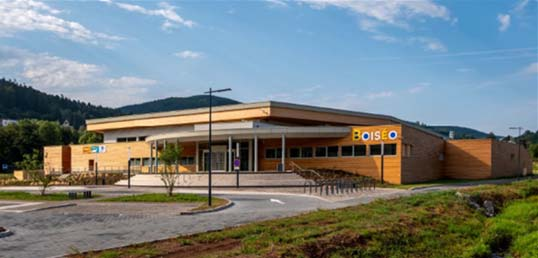
\includegraphics[width=0.7\linewidth]{img/fig001}
\end{center}
\label{fig001}
\caption{Complexe aquatique de la Broque}
\end{figure}

\vspace{-1cm}

\section{Pourquoi le savoir-nager est-il un enjeu préoccupant ? (15 min)}

\question{A partir du document technique DT1, lister les moments de la période de l'été 2018 où les pics de noyades sont les plus élevés. Préciser la particularité de cette année 2018.}

\question{À l'aide du document DT2, indiquer le nombre d'élèves concernés dans la communauté de communes de la vallée de la Bruche.}

\vspace{0.5cm}

Le projet Boiséo représente une opération d'envergure pour la CCVB, engageant la collectivité sur un projet destiné à couvrir les besoins de la population pour au moins les trois ou quatre prochaines décennies. Le bureau d'études IPK Conseil a dû tenir compte de nombreuses exigences lors de la conception de Boiséo.

Avant de démarrer toute installation et prévoir la sécurité dans un ERP (Établissement Recevant du Public), il est nécessaire de savoir à quelle catégorie le complexe aquatique se rapporte.

\newpage

Catégorie ERP en fonction de la capacité d'accueil :
\begin{itemize}
 \item Catégorie ERP 1 : à partir de 1 501 personnes,
 \item Catégorie ERP 2 : de 701 à 1 500 personnes,
 \item Catégorie ERP 3 : de 301 à 700 personnes,
 \item Catégorie ERP 4 : jusqu'à 300 personnes.
\end{itemize}

\question{Rechercher sur le document DT2 la capacité d'accueil du complexe
Boiséo. Indiquer la catégorie ERP correspondante.}

\question{À l'aide du document DT2, classer en trois catégories, sociale, économique et environnementale, les exigences contenues dans l'exigence principale \og Bassin de vie \fg id = \og 1 \fg.}

\question{Conclure sur les causes des noyades, le savoir nager comme mission prioritaire et comment le complexe aquatique Boiséo répond à ce besoin.}

\section{Comment faciliter l'accès des bassins aux personnes à mobilité réduite (P.M.R.) ? (20 min)}

En France, la loi n\textdegree\ 2005-102, du 11 février 2005, \og Loi pour l'égalité des droits et des chances, la participation et la citoyenneté des personnes handicapées \fg, vise à garantir une égalité de droits pour tous avec notamment la possibilité de se déplacer et d'accéder comme
tout un chacun aux services, commerces, équipements,...

Cette idée a été étendue aux personnes à mobilité réduite (P.M.R.). Les exigences à satisfaire sont décrites dans des arrêtés. Le document technique DT3 fournit des extraits de celui qui est actuellement en vigueur.

Les établissements recevant du public (E.R.P.), c'est-à-dire les magasins, bureaux, hôtels, piscines doivent être accessibles aux personnes en situation de handicap quel que soit celui-ci. Lors de la conception d'un bâtiment, comme le complexe aquatique Boiséo, des points de vigilance ont dû être définis pour rendre le bâtiment accessible à tous.

~\

\textbf{Étape 1, le parking:} comment créer des zones de stationnement adaptées ?

Le parking prévu pour ce complexe aquatique contient 3 places pour les bus, 120 places pour les véhicules légers, 8 emplacements pour les motos. Un parc à vélos composé de 20 supports en arceaux complète l'équipement du stationnement.

\question{À l'aide du document technique DT3, préciser comment la signalétique horizontale et verticale associée au stationnement d'une P.M.R. sont matérialisées (sur l'extrait du parking en bas du plan).}

\question{Calculer le nombre minimal de places adaptées à réserver aux P.M.R dans la zone de stationnement pour le public.}

\question{À partir de l'échelle indiquée sur le document technique DT3, mesurer la longueur et la largeur d'une place de stationnement pour P.M.R.
Calculer les dimensions réelles de la place de stationnement en mètres.}

\question{À l'aide du document DT3, conclure vis-à-vis du respect de l'arrêté du 20 avril 2017 sur les dimensions des places de parking.}

~\ \\

\textbf{Étape 2, le cheminement extérieur :} comment accéder sans effort et sans obstacle à l'entrée du bâtiment ?

\question{À partir du document technique DT3, relever les altitudes et la longueur de la zone 3. Calculer la pente, en pourcentage, de la zone 3. Justifier l'existence de la zone 4.}

\textbf{Étape 3 :} l'accès aux bassins respecte-t-il les normes ?

~\

Les usagers du centre aquatique, après s'être dévêtus et avoir pris une douche, vont accéder aux bassins en passant obligatoirement par un pédiluve.

\begin{figure}[ht!]
\begin{center}
 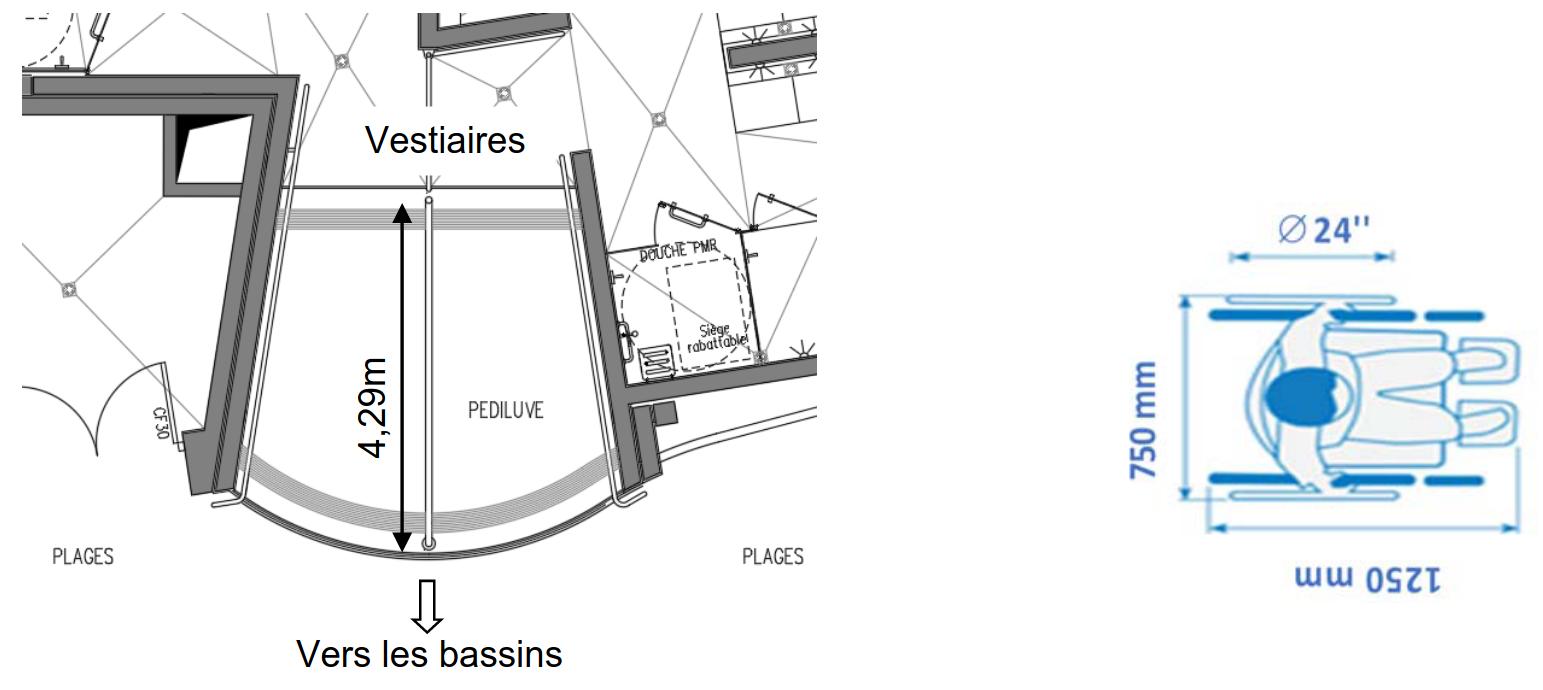
\includegraphics[width=0.6\linewidth]{img/fig002}
\end{center}
\label{fig002}
\caption{Dimensions pédiluve et gabarit fauteuil roulant}
\end{figure}

La figure ci-dessus donne le gabarit d'encombrement d'un fauteuil roulant. Une roue arrière de fauteuil a un diamètre de 24'' (pouces), soit 610 mm.

\question{Relever la longueur du pédiluve. Vérifier que cette longueur est supérieure ou égale à 2 tours de roue de fauteuil pour s'assurer qu'elles soient entièrement nettoyées.}

\section{Comment protéger les usagers contre les éléments climatiques ? (15 min)}

Un auvent couvre l'entrée du centre aquatique afin de limiter les effets de la neige et de la pluie sur les usagers.

\question{Grâce au document technique DT4, définir la fonction assurée par le poteau étudié.}

\question{Parmi les 4 sollicitations : traction, compression, flexion, torsion, indiquer celle que subit le poteau.}

\question{Calculer l'action permanente $G$ appliquée au poteau, à partir de $g$ et de $S$. Calculer l'action due à la neige $Sn$ appliquée au poteau, à partir de $sn$ et de $S$. Calculer l'intensité de la force $F$ appliquée au poteau.}

\question{En prenant $F = 37 kN$, calculer la contrainte $\sigma=\frac{F}{S}$ ($S$ étant la section) subie par le poteau. En déduire que le tube est correctement dimensionné en montrant que $\sigma<Re$.}

\section{Comment estimer les possibilités de récupération d'énergie solaire sur le toit de la piscine Boiséo et gérer le chauffage des bassins ? (20 min)}

\question{À l'aide du document technique DT5, calculer la surface maximale St en $m^2$ de toiture de la piscine Boiséo sur laquelle il est possible d'installer des panneaux solaires (toitures terrasse 1 + terrasse 2).}

\question{À partir du document technique DT6, relever la valeur de l'irradiance (rayonnement solaire) quotidienne moyenne en $kW\cdot h\cdot m^{-2}\cdot jour^{-1}$.}

\question{En prenant l'irradiance $I=3kW\cdot h\cdot m^{-2}\cdot jour^{-1}$ , et $St = 350 m^2$, calculer l'énergie quotidienne théorique totale $W_{tq}$ en $kW\cdot h\cdot jour^{-1}$ récupérable sur les toitures des deux terrasses.}

\question{En prenant $W_{tq}=1000 kW\cdot h\cdot jour^{-1}$, et sachant que les panneaux solaires thermiques ont un rendement moyen de 80 \%, calculer l'énergie quotidienne $W_{psth}$ en $kW\cdot h\cdot jour^{-1}$ récupérable par ces panneaux.}

La régulation de température de l'eau des bassins de la piscine se fait à l'aide de capteurs implantés sur le circuit d'eau des bassins et sur le circuit du fluide caloporteur des panneaux solaires thermiques. À partir de ces relevés, la source d'énergie est sélectionnée pour chauffer l'eau des bassins.

L'énergie thermique provenant des panneaux solaires thermiques est utilisée en permanence. Pour maintenir la température à une valeur constante, la pompe à chaleur vient compléter cet apport d'énergie de la manière suivante :
\begin{itemize}
 \item Si l'écart de température entre le fluide caloporteur des panneaux solaires thermiques et l'eau des bassins est inférieur ou égale à 50\textdegree C, la pompe à chaleur est à l'état \og MARCHE \fg pour compléter l'apport d'énergie,
 \item Si l'écart de température entre le fluide caloporteur des panneaux solaires thermiques et l'eau des bassins est supérieur à 50\textdegree C, la pompe à chaleur est à l'état \og ARRÊT \fg.
\end{itemize}

Remarque : le chauffage au gaz (chaudière à condensation), n'est utilisé que pour la mise en chauffe initiale des bassins.

Avec :
\begin{itemize}
 \item Tb = Température de l'eau des bassins en \textdegree C,
 \item Tcps = Température du liquide caloporteur des panneaux solaires thermiques,
 \item ChPC = Chauffage Pompe à Chaleur.
\end{itemize}

\question{Pour sélectionner la source d'énergie en fonction des températures de l'eau des bassins et du fluide caloporteur des panneaux solaires, compléter les zones grisées de l'algorigramme du document réponse DR2.}

\newpage

\section{Comment optimiser la gestion des énergies pour le chauffage de l'eau des bassins, de l'eau chaude sanitaire et des locaux ? (50 min)}

La piscine Boiséo a un besoin important en énergie thermique destinée à :
\begin{itemize}
 \item chauffer l'eau des bassins,
 \item chauffer l'eau chaude sanitaire (ECS) pour les douches, les lavabos, et le local du personnel,
 \item chauffer les locaux.
\end{itemize}

\question{Identifier sur le diagramme des exigences DT2 les 3 sources qui
alimentent la piscine en énergie. Préciser pour chacune d'elles s'il s'agit d'une énergie renouvelable ou non-renouvelable, d'une énergie primaire ou secondaire.}

\question{De ces trois sources d'énergie, préciser celle qui devrait être mise en \oe uvre en priorité et pour quelles raisons.}

~\

La production d'énergie thermique est assurée par 3 systèmes :
\begin{itemize}
 \item des panneaux solaires thermiques posés horizontalement sur le toit du bâtiment, d'une puissance de 45 kW,
 \item trois pompes à chaleur (PAC) d'une puissance totale de 75 kW,
 \item une chaudière à gaz d'une puissance de 700 kW.
\end{itemize}

\question{Calculer la puissance maximum PMAX que peuvent fournir ces trois modes de chauffage lorsqu'ils fonctionnent en même temps.}

~\

En fonctionnement nominal, c'est-à-dire pour maintenir la température de l'eau dans le bassin et chauffer les locaux, la consommation est de 300 kW. Cette puissance est prioritairement fournie par les panneaux solaires thermiques et les pompes à chaleur.

\question{Calculer dans ce cas la puissance P ch que doit fournir la chaudière à gaz. Déterminer la marge de puissance P Marge restant pour la chaudière à gaz.}

~\

La piscine est alimentée en eau par le réseau public. L'eau arrive à une température de 12\textdegree C. Les bassins contiennent $660m^3$ d'eau.
Lors du remplissage des bassins, il faut chauffer l'eau pour qu'elle puisse atteindre sa température nominale de 28\textdegree C.
On rappelle que : $W = \Delta\theta\cdot m\cdot Cp$, avec:
\begin{itemize}
 \item $\Delta\theta$ : différence de température en \textdegree C,
 \item $m$ : masse de l'eau en kg,
 \item $Cp$ : chaleur massique de l'eau ($4185J\cdot kg^{-1}\cdot\degree C^{-1}$)
 \item $W$ : énergie en Joule (1 Joule=1 Watt seconde),
 \item $1m^3$ d'eau a une masse de $1000 kg$.
\end{itemize}

\question{Calculer la quantité d'énergie thermique W th qu'il faut fournir pour chauffer l'eau. Exprimer ce résultat en Joule puis en $kW\cdot h$.}

On prendra une puissance disponible pour chauffer l'eau de $500 kW$.

\question{Déterminer le temps en heures nécessaire à la montée en température de l'eau.}

\newpage

On montre que l'équation différentielle qui régit la chauffe de l'eau à partir des échanges avec un fluide circulant dans un circuit de chauffe est:

\begin{center}
$\frac{m\cdot Cp}{h\cdot S}\cdot\frac{dt_e(t)}{dt}+t_e(t)=T_{fluide}$
\end{center}

Avec: 
\begin{itemize}
 \item $S$ la surface d'échange entre le serpentin et l'eau : $S = 30 m^2$,
 \item $h$ Coefficient d'échange conducto-convectif dans le cas étudié : $h=3000W\cdot m^{-2}\cdot K^{-1}$,
 \item $T_{fluide}$ température du liquide de chauffe : $T_{fluide}=90\degree$,
 \item $t_e(t)$ température de l'eau à chauffer.
\end{itemize}

\question{Passer cette équation dans le domaine de Laplace et déterminer $T_e(p)=L[t_e(t)]$ en fonction des autres paramètres. Montrer qu'on peut écrire $T_e(p)=\frac{b}{p\cdot\left(p+a\right)}+\frac{c}{p+a}$, en déduire $a$, $b$ et $c$.}

\question{Montrer que l'on peut écrire $T_e(p)=\frac{\frac{b}{a}}{p}+\frac{c-\frac{b}{a}}{p+a}$.}

\question{En déduire $t_e(t)$ en fonction de $a$, $b$ et $c$ et si vous avez trouvé la réponse à la question \ref{q27} en fonction de $m$, $Cp$, $h$, $S$ et $T_{fluide}$.}

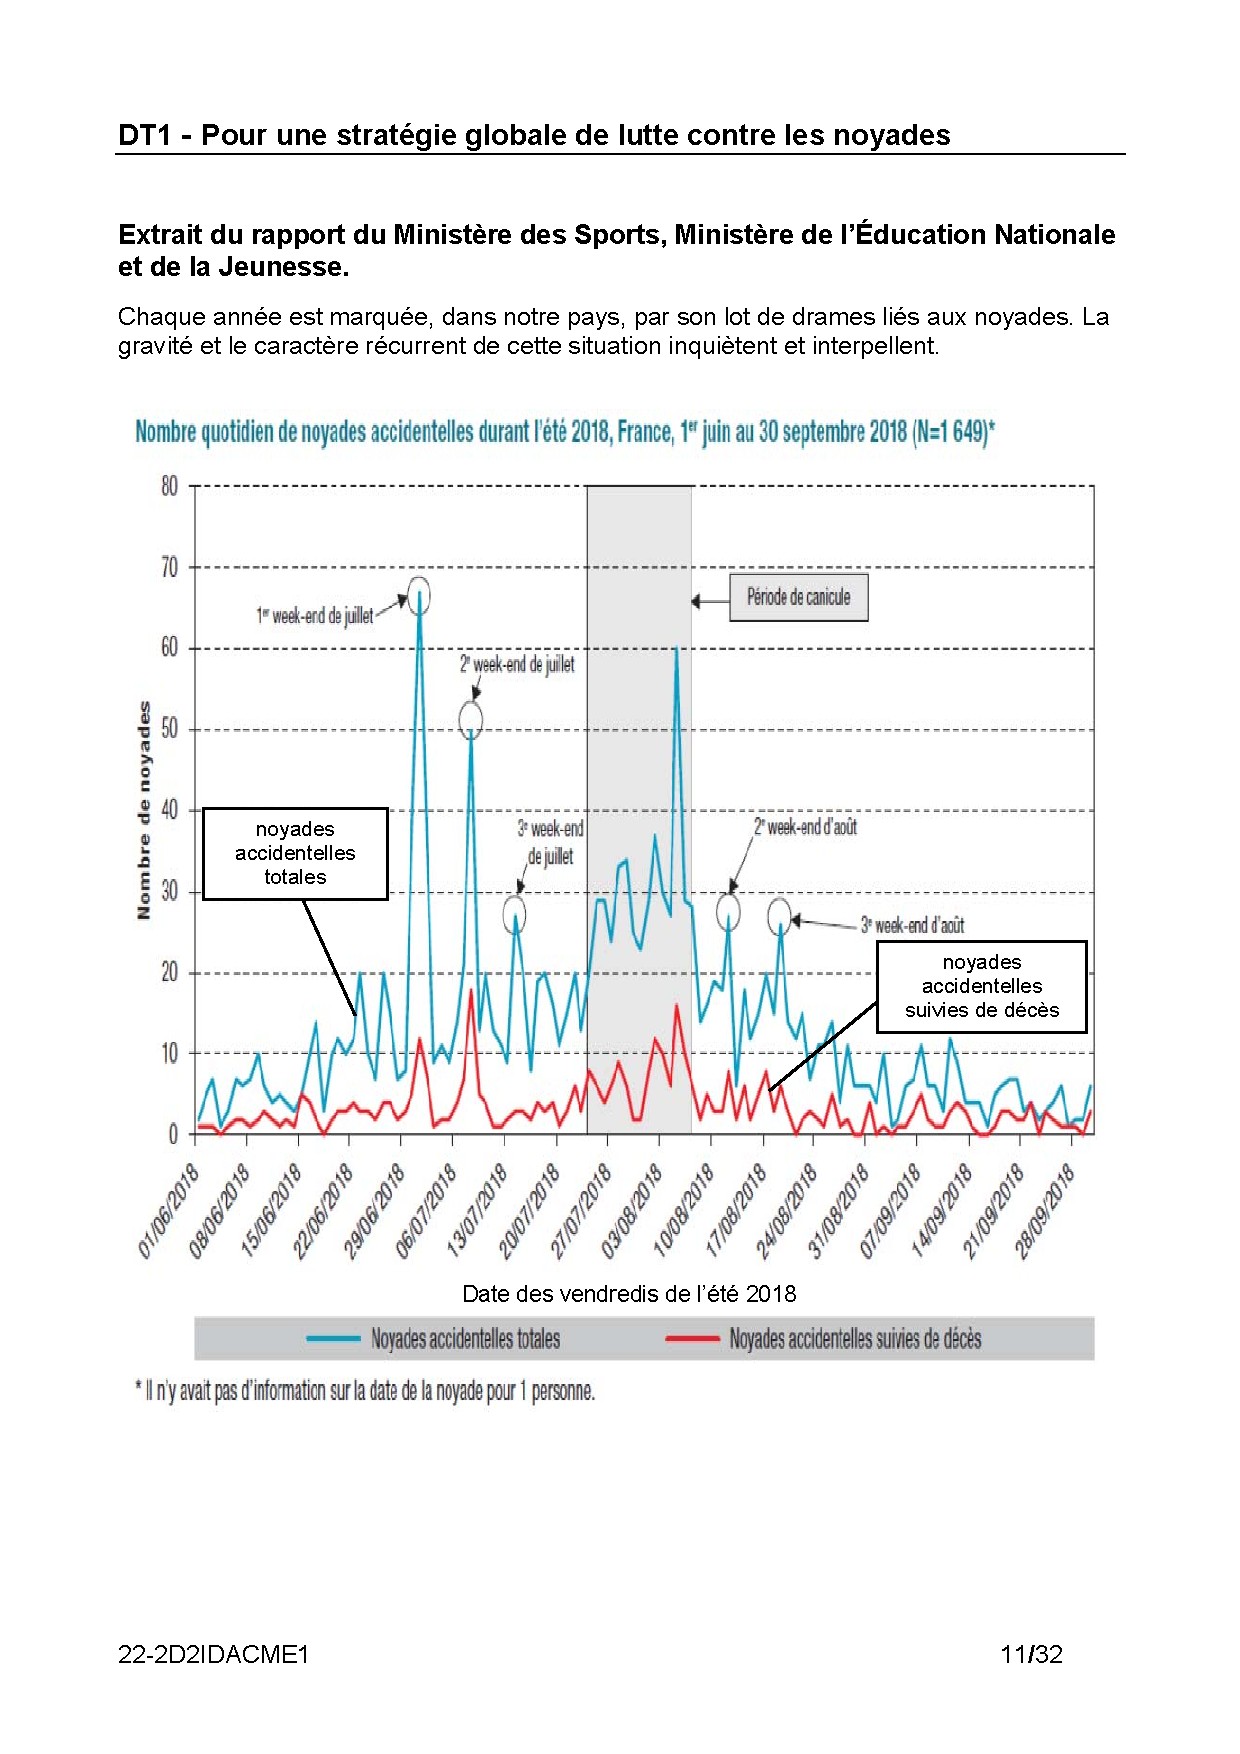
\includepdf[offset=5mm -10mm 0mm 0mm,pages=1-6]{annexes.pdf}

\cleardoublepage ~\ \cleardoublepage

\ifdef{\public}{\pagestyle{documentreponse}}{\pagestyle{correction}}

\reponse{4}{}{Les noyades interviennent majoritairement les week-ends de l'été, notamment les premiers de juillet. Il y en a aussi beaucoup durant la période de canicule de fin juillet à début août.}

\reponse{2}{}{Il y a 3265 élèves.}

\reponse{2}{}{La capacité max est de 700 personnes, c'est donc un ERP3.}

\reponse{3}{}{\begin{itemize}
 \item \og Social \fg : id 1.1, 1.2, 1.3, 1.8,
 \item \og Economique \fg : id 1.7,
 \item \og Environnemental \fg : id 1.4, 1.5, 1.6.
\end{itemize}}

\reponse{3}{}{Le manque de structure pour apprendre la natation fait que les enfants et certains adultes ne savent pas nager. Afin de diminuer le nombre de noyades, il faut avant l'été permettre au maximum de personnes d'avoir accès à une piscine. Le but de ce complexe est justement d'y faciliter l'accès à tous quelque soit l'âge ou les capacités physiques.}

\reponse{2}{}{Un panneau et des marquages au sol permettent cette matérialisation.}

\reponse{2}{}{Le nombre de place doit être supérieur à $120\cdot 2\%=\frac{120\cdot 2}{100}=2.4$. Il faut donc 3 places.}

\reponse{2}{}{Largeur: $19mm \rightarrow 19\cdot 180=3420mm=3.42m$, Longueur: $28mm \rightarrow 28\cdot 180=5040mm=5.04m$}

\reponse{2}{}{Le cahier des charges est respecté car $3.42m>3.3m$ et $5.04m>5m$.}

\reponse{2}{}{On passe de $325.62m$ à $325.18m$ en $9.16m$, la pente est donc $\frac{325.62-325.18}{9.16}=\frac{0.44}{9.16}\leq 5\%$. La pente est de plus de 4\% mais comme la longueur est inférieure à 10m, il n'est pas nécessaire de placer un palier. Il en faut simplement un avant ou après.}

\reponse{2}{}{La longueur du pédiluve est de $4,29m$, deux tours de roues font $0,61\cdot \pi\cdot 2\approx 0,61\cdot 3,14\cdot 2\approx 0,6\cdot 3,2\cdot 2\approx 3,84m$, donc la longueur du pédiluve est suffisante.}

\ifdef{\public}{\newpage}

\reponse{2}{}{Le poteau porte la toiture.}

\reponse{2}{}{Le poteau est soumis à de la compression.}

\reponse{3}{}{$G=0.28\cdot 34.76\approx 0.3\cdot 34\approx 10.2kN$ \\ $Sn=0.45\cdot 34.76=17.38-1.738\approx 15.64kN$ \\ $F=1.35\cdot G+1.5\cdot Sn=1.35\cdot 10.2+1.5\cdot 15.64=1.35\cdot 10.2+1.5\cdot 15.64=13.8+23=36.8kN.$}

\reponse{2}{}{$\sigma=\frac{37\cdot 10^3}{2703}\approx \frac{36.9\cdot 10^3}{2700}\approx \frac{4.1\cdot 10}{3}\approx 13Mpa<235$. Le tube est largement dimensionné.}

\reponse{2}{}{$St=St1+St2$

$St1=23.79\cdot 10.48\approx 23.8\cdot 10.5\approx 238+11.9\approx249.9m^2$

$St2=15.07\cdot 8.25\approx 120+3.75\approx 123.75m^2$

$St=249.9+123.75=373.65m^2$
}

\ifdef{\public}{\newpage}

\reponse{2}{}{Irradiance$=3.05kW\cdot h\cdot m^{-2}\cdot jour^{-1}$}

\reponse{2}{}{$W_{tq}=3\cdot 350=1050kWh\cdot jour^{-1}$}

\reponse{2}{}{$W_{tq}=1000\cdot 0.8=800kWh\cdot jour^{-1}$}

\reponse{0}{\begin{center}
 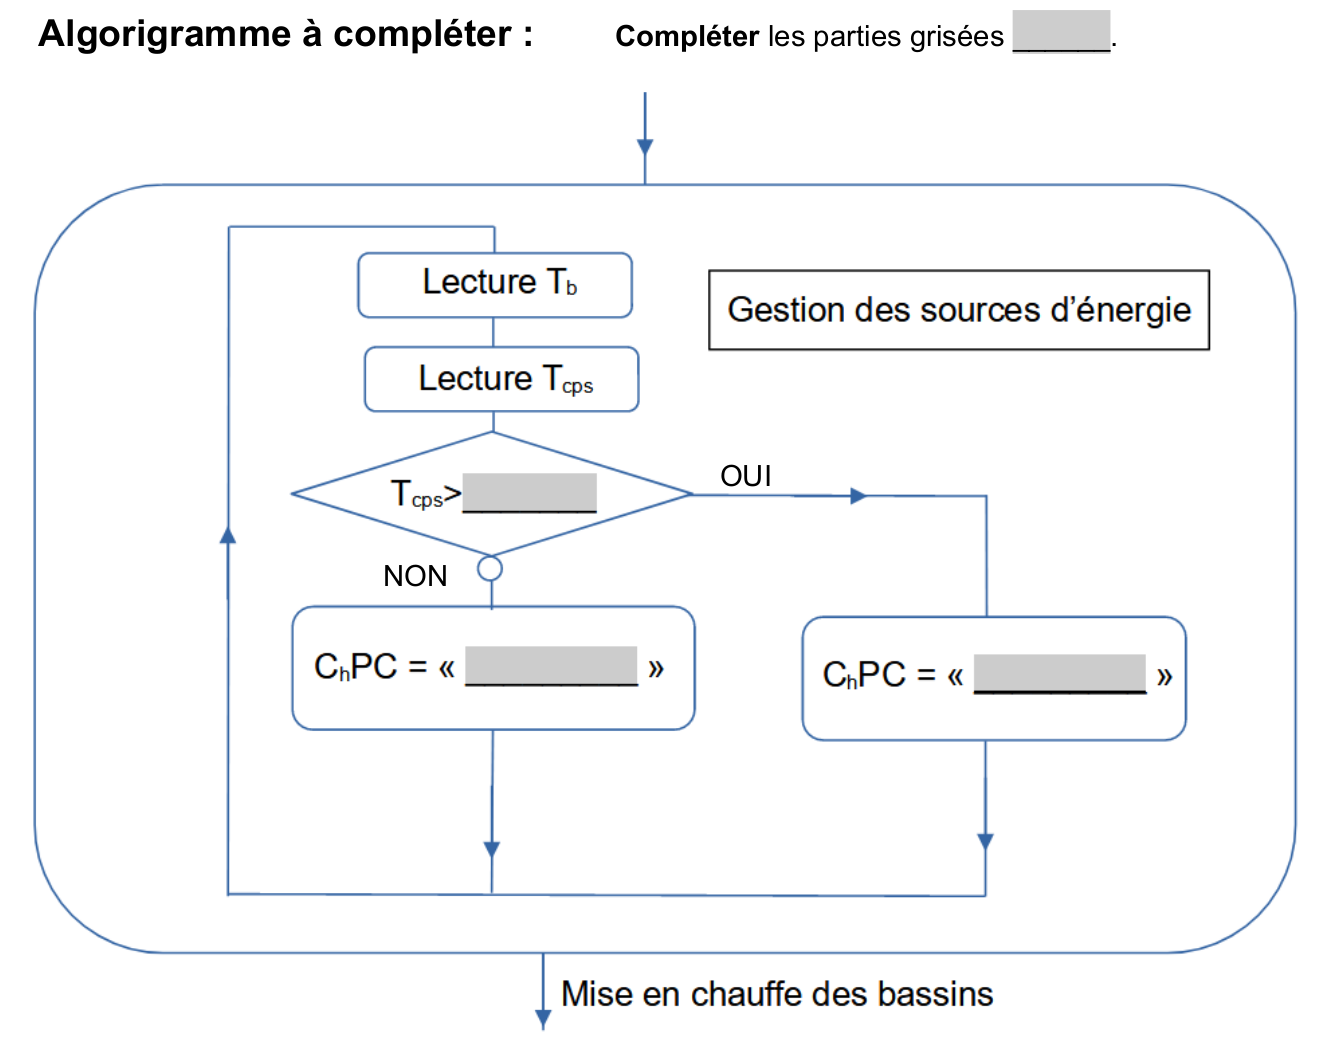
\includegraphics[width=0.65\linewidth]{img/fig003}
\end{center}
\label{fig003}
}{
\begin{center}
 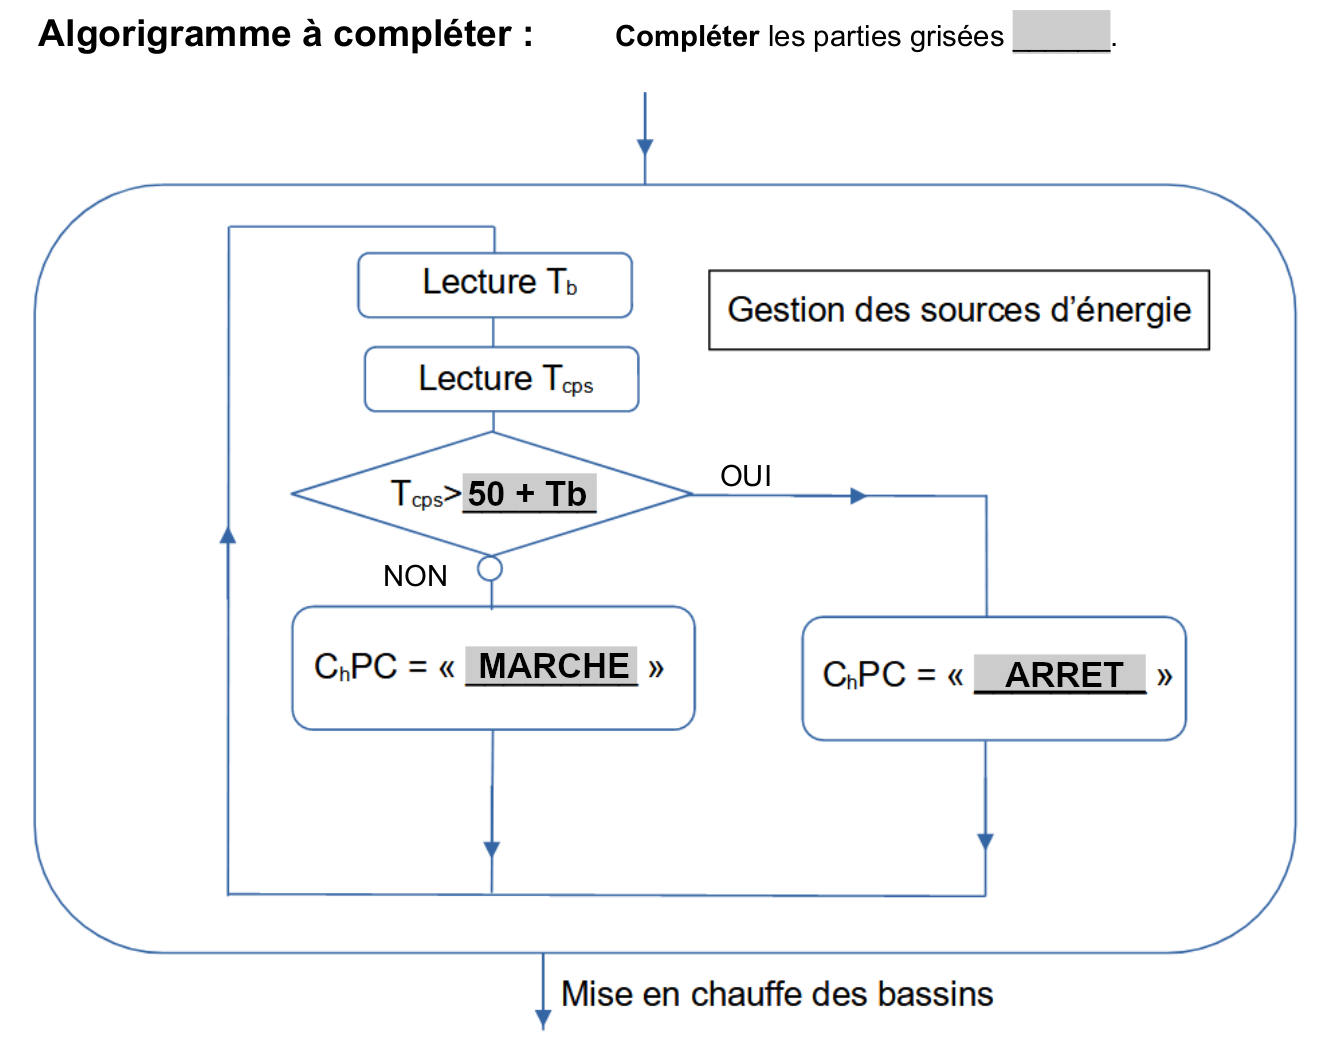
\includegraphics[width=0.65\linewidth]{img/fig003_cor}
\end{center}
\label{fig003}
}

\ifdef{\public}{\newpage}

\reponse{2}{}{\begin{itemize}
\item Gaz: énergie primaire non renouvelable,
\item Solaire: énergie primaire renouvelable,
\item Electricité: énergie secondaire et non renouvelable. 
\end{itemize}}

\reponse{2}{}{L'énergie solaire est renouvelable, elle devrait donc être mise en \oe uvre en priorité.}

\reponse{2}{}{$P_{max}=45+75+700=820kW$}

\reponse{2}{}{$P_{ch}=300-45+75=180kW$, il reste une marge de $520kW$.}

\reponse{2}{}{$W=\Delta\theta\cdot m\cdot Cp=(28-12)\cdot 660\cdot 1000\cdot 4185\approx 16\cdot 66 \cdot 42 \cdot 10^6\approx 2^5\cdot 14 \cdot 10^8\approx 448 \cdot 10^8J$, soit $\frac{448\cdot 10^8}{3600\cdot 1000}=\frac{112\cdot 10^8}{9\cdot 10^5}\approx 12\cdot 10^3kWh.$}

\reponse{2}{}{Il faut $\frac{12000}{500}=24$ heures.}

\ifdef{\public}{\newpage}

\reponse{5}{}{
$\frac{m\cdot Cp}{h\cdot S}\cdot \left(p\cdot T_e(p)-t_0\right)+T_e(p)=\frac{T_{fluide}}{p}$

$\frac{m\cdot Cp}{h\cdot S}\cdot p \cdot T_e(p)+T_e(p)=\frac{T_{fluide}}{p}+t_0\cdot \frac{m\cdot Cp}{h\cdot S}$

$T_e(p)=\frac{\frac{T_{fluide}}{p}+t_0\cdot \frac{m\cdot Cp}{h\cdot S}}{\frac{m\cdot Cp}{h\cdot S}\cdot p+1}=\frac{\frac{T_{fluide}}{p}\cdot \frac{h\cdot S}{m\cdot Cp}+t_0}{p+\frac{h\cdot S}{m\cdot Cp}}=\frac{T_{fluide}\cdot \frac{h\cdot S}{m\cdot Cp}}{p\cdot\left(p+\frac{h\cdot S}{m\cdot Cp}\right)}+\frac{t_0}{p+\frac{h\cdot S}{m\cdot Cp}}$

\begin{itemize}
 \item $a=\frac{h\cdot S}{m\cdot Cp}$,
 \item $b=T_{fluide}\cdot \frac{h\cdot S}{m\cdot Cp}$,
 \item $c=t_0$.
\end{itemize}
}

\reponse{5}{}{$T_e(p)=\frac{b}{p\cdot\left(p+a\right)}+\frac{c}{p+a}=\frac{A}{p}+\frac{B}{p+a}+\frac{c}{p+a}=\frac{A\cdot p+A\cdot a+B\cdot p}{p\cdot\left(p+a\right)}+\frac{c}{p+a}$

On a ainsi:
\begin{itemize}
 \item $A+B=0$, donc $B=-A$,
 \item $A\cdot a=b$, donc $A=\frac{b}{a}$.
\end{itemize}

$T_e(p)=\frac{\frac{b}{a}}{p}-\frac{\frac{b}{a}}{p+a}+\frac{c}{p+a}=\frac{\frac{b}{a}}{p}+\frac{c-\frac{b}{a}}{p+a}$
}

\reponse{5}{}{$t_e(t)=\frac{b}{a}+\left(c-\frac{b}{a}\right).e^{-a\cdot t}$

Pour ceux qui sont trouvé les expressions littérales de $a$, $b$ et $c$.

$t_e(t)=T_{fluide}+\left(t_0-T_{fluide}\right).e^{-\frac{h\cdot S}{m\cdot Cp}\cdot t}$
}

\end{document}
